\documentclass{article}
\usepackage{amsmath}
\usepackage{amssymb}
\usepackage{amsthm}
\usepackage{verbatim}
\usepackage{graphicx}
\usepackage{caption}
\usepackage{subfig}

%\usepackage{caption}
%\usepackage{epstopdf}
%\usepackage{float}


\newtheorem{theorem}{Theorem}
%\numberwithin{theorem}{subsection}

\theoremstyle{definition}
\newtheorem{exmp}{Example}
\numberwithin{exmp}{subsection}





\title{Exploring Bounds}
\author{Tyler Friedman}


\begin{document}
\maketitle

\section{Introduction}

An interesting problem in coding theory is determining the maximum
number of codewords in a code with certain parameters.  For an $n$-dimensional code, we are interested in 
the maximum number of codewords such that the code has minimum distance $d$.  
Formally, we use the notation $A_q(n,d)$
and $B_q(n,d)$ to define the maximum of number of codewords in a code over
$\mathbb{F}_q$ of length $n$ and minimum distance $d$ for an arbitrary (linear
on non-linear) code and linear code, respectively.  

For arbitrary $n$ and $d$, it is difficult to find $A_q(n,d)$ and $B_q(n,d)$ exactly.
 In lecture, we have considered upper bounds---Sphere Packing, Singleton, and Greismer---as well as
lower bounds---Gilbert and Varshamov---on these values.  The purpose of this
paper is to take a survey of other well-known bounds in the literature that we have not discussed.  
In the first part of the paper, we will consider the Plotkin Upper bound, 
the Elias Upper bound, and the Linear Programming Upper Bound.  In the second part of the paper, we will consider asymptotic versions
of Singleton, Plotkin, Hamming, and Elias.  (I am very certain that I won't get to discuss all of these bounds, but I am currently unsure how much space each discussion will take up so I've
listed all that I am considering.)  For each bound, we will consider its proof as well
as related examples.  Lastly, in the final part we will consider lexicodes, an interesting subset of linear codes that meet the Gilbert Bound.

Some implementation specific details: for the Linear Programming bound, I will introduce basic linear programming concepts and as well as the Krawtchouck polynomials.  For the 
Asymptotic Hamming bound I will introduce the Hilbert entropy function.  


\section{Upper Bounds}

\subsection{Plotkin Upper Bound}
%Plotkin
%talk about importance
%define it
%prove it
%work out some examples

The Plotkin Bound is an upper bound that often improves upon the Sphere Packing Bound on $A_q(n,d)$.

\begin{theorem}[Plotkin]
Let $C$ be an $(n,M,d)$ code over $\mathbb{F}_q$ such that $rn < d$ where $r = 1 - q^{-1}$.  Then
\begin{equation}
A_q(n,d) \le \left \lfloor \frac{d}{d-rn}\right\rfloor
\end{equation}
\end{theorem}

Before proving this bound, it is important to note that it is only valid when $d$ is sufficiently close to $n$.  For large $q$, this is can be a considerable limiting factor.
Consider that our restriction is $n<2d$ for $q=2$, $n<\frac{3}{2}d$ for $q=3$, $n<\frac{4}{3}d$ for for $q=4$, etc.


\begin{proof}
Let 
\begin{equation} \label{plotkin_1}
S = \sum_{x \in \mathcal{C}} \sum_{y \in \mathcal{C}} \text{d}(x,y)
\end{equation}

Note that for $x,y \in \mathcal{C}$, d$(x,y)=0$ for $x=y$, and $d \le$ d$(x,y)$ for $x\neq y$.  This implies that
\begin{equation} \label{plotkin_1_5}
M(M-1)d\le S
\end{equation}

This comes directly from equation \ref{plotkin_1}.  We have $M$ possible codewords to consider for $x$ in the outer summation, $M-1$ distinct codewords from $x$ to consider in the inner summation for $y$, 
and the distance between $x$ and $y$ will always be greater than or equal to the minimum distance $d$.

Next, let $\mathcal{M}$ be the $M \times n$ matrix whose rows are the codewords of $\mathcal{C}$.  For $1 \le i \le n$, let $n_{i,\alpha}$ be the number of times $\alpha \in
 \mathbb{F}_q$ occurs in column $i$ of $\mathcal{M}$.  Note that $\sum_{\alpha \in \mathbb{F}_q} n_{i,\alpha} = M$ for $1\le i \le n$.  This is simply because there are $M$ total
 elements of $\mathbb{F}_q$ in each column, so the sum over all $n_{i,\alpha}$ must necessarily be $M$.  

I claim that we can rewrite $S$ as a double sum over these $n_{i,\alpha}$ values.  Specifically,

\begin{equation}
S = \sum_{i=1}^{n} \sum_{\alpha\in\mathbb{F}_q} n_{i,\alpha}(M - n_{i,\alpha}).
\end{equation}

Note that $n_{i,\alpha}(M - n_{i,\alpha})$ is multiplying the number of times $\alpha$ occurs in column $i$ by the number of times it doesn't occur in column $i$.  In other words, we're counting the number of times two elements of the same
column are not equivalent, exactly the condition that constitutes our Hamming distance.   By summing over all $\alpha$ and then all columns, we arrive at the same value generated by \ref{plotkin_1}.

Next, simplify:

\begin{equation}
\begin{split}
\sum_{i=1}^{n} \sum_{\alpha\in\mathbb{F}_q} n_{i,\alpha}(M - n_{i,\alpha}) &= M\sum_{i=1}^{n} \sum_{\alpha\in\mathbb{F}_q} n_{i,\alpha} - \sum_{i=1}^{n} \sum_{\alpha\in\mathbb{F}_q} n_{i,\alpha}^2 \\
&= nM^2 - \sum_{i=1}^{n} \sum_{\alpha\in\mathbb{F}_q} n_{i,\alpha}^2
\end{split}
\end{equation}

Recall the Cauchy-Schwarz inequality, which states that $\left(\sum_{i=1}^n x_i y_i \right )^2 \le \left(\sum_{i=1}^n x_i^2 \right ) \left(\sum_{i=1}^n y_i^2 \right )$
For our purposes, this means that $\left(\sum_{\alpha\in\mathbb{F}_q} 1\cdot n_{i,\alpha} \right )^2 \le q \left(\sum_{\alpha\in\mathbb{F}_q} n_{i,\alpha}^2 \right )$.

Using this inequality, we obtain

\begin{equation} \label{plotkin_2}
S \le nM^2 - \sum_{i=1}^n q^{-1} \left(\sum_{\alpha\in\mathbb{F}_q} 1\cdot n_{i,\alpha} \right )^2 = nM^2 - \frac{nM^2}{q} = nrM^2.
\end{equation}

Combining \ref{plotkin_1_5} and \ref{plotkin_2}, we get $M(M-1)d \le nrM^2$, which simplifies to 

\begin{equation}
M \le \left\lfloor \frac{d}{d-rn} \right\rfloor.
\end{equation}

\end{proof}

It is interesting to see exactly how the Sphere Packing and Plotkin bounds compare for specific values of $n$ and $d$.  For the following examples we will assume $q=2$.    
Also, recall that if $d$ is even, $A_2(n,d) = A_2(n-1,d-1)$.  

\begin{exmp}
$(n,d) = (7,4)$.

Applying the Sphere Packing bound, we have $A_2(7,4) = A_2(6,3) \le \frac{2^6}{1 + 6}$, 
giving us $A_2(7,4) \le \textbf{9}$.

Applying the Plotkin bound, we have $A_2(7,4) \le \frac{4}{4-\frac{1}{2}\cdot7} = \textbf{8}$.

\end{exmp}

\begin{exmp}
$(n,d) = (9,6)$.

Applying Sphere Packing, we have  $A_2(9,6) = A_2(8,5) \le \frac{2^8}{1+8+28}$, giving us $A_2(n,d) \le \textbf{6}$.

Applying the Plotkin bound, we have $A_2(9,6) \le \frac{6}{6-\frac{1}{2}\cdot9} = \textbf{4}$.
\end{exmp}

It is also interesting to consider a more broader picture of what is going on here.  Below is a graph comparing rates of codes versus the Sphere Packing and Plotkin bounds
that we can calculate for those values for different values of q.  

\begin{comment}
\begin{figure}
\begin{subfigure}{.5\textwidth}
  \centering
  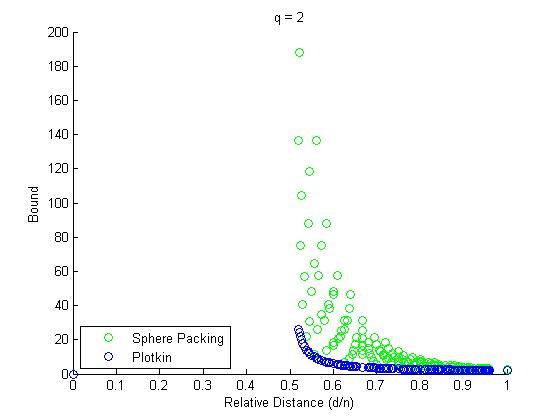
\includegraphics[width=.8\linewidth]{plotkin_q2.png}
  \caption{1a}
  \label{fig:sfig1}
\end{subfigure}%
\begin{subfigure}{.5\textwidth}
  \centering
  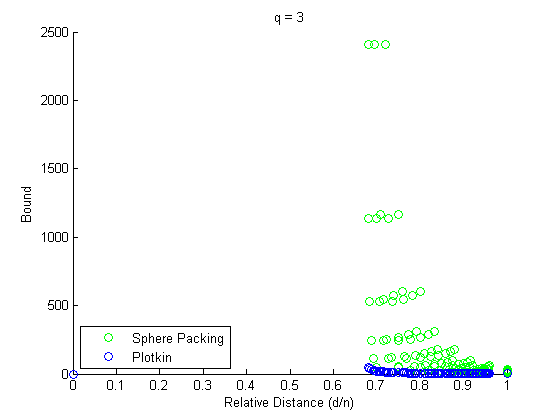
\includegraphics[width=.8\linewidth]{plotkin_q3.png}
  \caption{1b}
  \label{fig:sfig2}
\end{subfigure}
\caption{plots of....}
\label{fig:fig}
\end{figure}
\end{comment}


\section{Lexicodes}
We end our discussion on bounds with an interesting class of linear codes
called Lexicodes.  


\section{Asymptotic Bounds}
We now wish to consider these $A_q(n,d)$ values as n goes to infinity.  To do so, we must more formally define two terms.

In class, we have considered the \textit{rate} of a linear code, $k/n$, as one measure of the goodness of a code.  That is,
the rate tells us how much information relative to redundancy that our codewords provide.  The concept of rate can be generalized
to non-linear codes as well.  For a possibly nonlinear code over $\mathbb{F}_q$ with $M$ codewords, the \textit{rate} is defined to be $n^{-1} \log_q {M}$.  Notice that
for an $[n,k,d]$ linear code, $M = q^k$ and hence the rate is $k/n$ as we expect.

A second notion of goodness that we have discussed, but I think not formally defined, is the \textit{relative distance} of a code.  For a linear or nonlinear code of length n
has minimum distance d, this value is the ratio $d/n$. 

Consequently, for our asymptotic bounds, we are interested in the largest possible rate for a family of codes over $\mathbb{F}_q$ of lengths going to infinity with relative 
distances approaching some constant $\delta$.  In other words, we consider the equation:

\begin{equation}
\alpha_{q}(\delta) = \limsup_{n \to \infty} n^{-1} \log_q A_q(n,\delta n)
\end{equation}


[What does this imply?]

\subsection{Asymptotic Singleton Bound}

Recall the Singleton Bound from lecture:

\begin{theorem}
For $d \le n$, $A_q(n,d) \le q^{n-d+1}$.
\end{theorem}

[explain what this means, what are the implications]


\begin{theorem}
If $0 \le \delta \le 1$, then $\alpha_q(\delta) \le 1 - \delta$.
\end{theorem} 
This theorem follows directly from the Singleton bound.

\begin{proof}
\begin{equation} 
\begin{split}
\alpha_{q}(\delta) & = \limsup_{n \to \infty} n^{-1} \log_q A_q(n,\delta n) \\
& \le \limsup_{n \to \infty} n^{-1} \log_q q^{n-\delta n+1} \\
& \le \limsup_{n \to \infty} \frac{n-\delta n+1}{n} \\
& \le 1 - \delta
\end{split}
\end{equation}
\end{proof}

\subsection{Asymptotic Plotkin Bound}



%First explore linear programming bound
Asymptotic singleton, include 2 examples
Asymptotic plotkin, some examples
draw graph
Asymptotic hamming
	define hilbert, prove 135,136, define vq(n,a),
	black box 2.10.3, prove 2.10.5


Table of common$a_q(n,d)$ values
Recall basic theory: thm 2.1.2, 2.1.6

Sections


Elias
talk about importance
define it
prove two lemmas that do the heavy lifting
easy proof to finish it off
work out some examples

Linear Programming Bound
talk about importance
define it
prove it
work out some examples


Note existence of two lower bounds, say we talked about them in class


\end{document}
